  %-----------------------------------------------
% DOCUMENT PACKAGES
%-----------------------------------------------
\documentclass[10pt]{article}
\usepackage[utf8]{inputenc}
\usepackage[T1]{fontenc}
\usepackage{graphics} %inclusion de figures
\usepackage{graphicx} %inclusion de figures
\usepackage{pstricks,pst-node} %Graphiques
\usepackage{tikz} %Tikz !
\usepackage[margin=1.3in]{geometry}
\usepackage[colorlinks=true,linkcolor=black,linktoc=all]{hyperref}
\usepackage[french]{babel}
\usepackage[small, sc, bf, center]{titlesec}
%Packages mathématiques
\usepackage{amsmath} %Equations
\usepackage{amssymb}
\usepackage{amsfonts}
\usepackage{pifont}
%Packages Tableaux
\usepackage{tabularx} %Tableaux
\usepackage{multirow} %Gestion des lignes
\usepackage{multicol} %Gestion des colones
\usepackage{arydshln} %Lignes en pointillés
\usepackage{fancybox} %Boites
\usepackage{multicol} %Colonnes
\usepackage{array} %Tableaux maths
\usepackage{fancybox}

\usepackage{cleveref}
\usepackage{fancyhdr}
\usepackage{tkz-graph}
\usepackage{csvsimple}
\usepackage{listings}
%\usepackage{subcaption}
%\usepackage{multicol}
%-----------------------------------------------
% DOCUMENT CONFIG
%-----------------------------------------------

% graphicx
\graphicspath{ {images/} }
% Add point after title number
\titleformat{\section}[block]{\sc\bfseries\center\large}{\thesection.}{0.5em}{}
\titleformat{\subsection}[block]{\sc\bfseries\center}{\thesubsection.}{0.5em}{}
\titleformat{\subsubsection}[block]{\sc\bfseries\center}{\thesubsubsection.}{0.5em}{}
% Page number reformat
\pagestyle{fancy}
\fancyfoot[C]{--~\thepage~--}
% Deactivate fancyhdr header
\renewcommand{\headrulewidth}{0pt}
\fancyhead{}
% tikz
\tikzstyle{vertex}=[circle, draw, inner sep=0pt, minimum size=6pt]
\newcommand{\vertex}{\node[vertex]}
\usetikzlibrary{arrows,petri,topaths,calc}
% listing style
\lstset{
frame=single,
basicstyle=\ttfamily\small,
numbers=left,
%numbersep=5pt,
%font=\ttfamily
}
\newcommand\tab[1][0.65cm]{\hspace*{#1}}
%-----------------------------------------------
% DOCUMENT BODY
%-----------------------------------------------
\begin{document}
\begin{center}
	\textbf{\huge Projet de FOSYMA\\[.5cm] Wumpus Multi-agent}\\[.5cm]
	\vspace{1.5cm}
	\textit{\Large B.Thanh Luong, Gualtiero Mottola}\\
	\vspace{1.5cm}
	
\includegraphics{logo}
	\vspace{1.5cm}
	\tableofcontents
\end{center}

\newpage

\section{Introduction}
	Ce projet consiste à développer une version multi-agent d'un jeu fortement inspiré de "Hunt the Wumpus"  cette variante du jeu est définie de la façon suivante : un ensemble d'agents en coopération sont placé dans un environnement inconnu. Ils ont pour mission d'explorer cet environnement et de récupérer un maximum de trésors qui sont disséminés dans cet environnement. Un agent Wumpus se trouve également dans l'environnement, il se déplace aléatoirement et a pour but de gêner l'exploration et la récupération des trésors.
	
\section{Présentation des Agents}
	Les trois type d'agent utilisables pour récolter un maximum de trésors sur la carte sont les suivants : les Agents Explorateurs qui n'ont pas la possibilité de récupérer des ressources, leur seul but est d'explorer la carte, des Agents Collecteurs qui ont un sac à dos correspondant a un type de trésor (\texttt{TREASURE} ou \texttt{DIAMONDS}) et qui ont une méthode permettant de récupérer ce type de trésor et le placer dans leur sac si celui-ci n'est pas plein. On note que lorsque cette action est exécutée une partie du trésor est perdue. Enfin le dernier type d'agent, l'agent Tanker qui ne peut pas ramasser de trésor mais a un sac à dos de capacité illimitée, tous les agents collecteurs ont la possibilité de donner leurs trésors à l'agent tanker. Ce sont les quantités présentes dans l'agent Tanker qui seront comptabilisées à la fin de l'exécution.

	\subsection{Comportement des Agents}
	Les comportements de nos trois types d'agents sont tous implémentés sous la forme de \texttt{FSMBehaviours} qui sont des diagrammes états-transitions (state chart). La classe offre des méthodes pour enregistrer les états et les transitions qui définissent l'ordre des behaviours.	Chaque état du FSM est un behaviour qui est exécuté selon l'ordre définit par l'utilisateur.\\
	\tab Nous allons décrire dans cette section le comportement principal de chaque agent, puis dans la section suivante la suite de behaviours qui leur permet de communiquer et qui est identique pour tous les types d'agents. Le behaviour Main est le comportement principal de chaque agent, nous avons \texttt{ExploreBehaviour} pour les Agents Explorateurs, \texttt{CollectBehaviour} pour les agents Collecteurs, etc.. En général dans ce comportement, l'agent se déplace, collecte le trésor dans la case où il se trouve ou même ne rien fait mais surtout pas la communication avec les autres.

\begin{lstlisting}
FSMBehaviour fsmBehaviour = new FSMBehaviour();
fsmBehaviour.registerFirstState(new MainBehavior(this),"Main");
fsmBehaviour.registerState(new CheckMailBehavior(this),"Ckm");
fsmBehaviour.registerState(new RequestConnectionBehaviour(this),"Com");
fsmBehaviour.registerState(new SendMapBehaviour(this),"Smp");
fsmBehaviour.registerState(new ReceiveMapBehaviour(this),"Rmp");

fsmBehaviour.registerTransition("Main","Ckm",1); //main to check mail

fsmBehaviour.registerTransition("Ckm","Com",1); //check mail to start com
fsmBehaviour.registerTransition("Ckm","Smp",2); //check mail to send map

fsmBehaviour.registerTransition("Com","Rmp",1); //com to receive

fsmBehaviour.registerTransition("Smp","Rmp",1); // send to receive
fsmBehaviour.registerTransition("Smp","Main",2); // send to main

fsmBehaviour.registerTransition("Rmp","Main",1); // receive to explore
fsmBehaviour.registerTransition("Rmp","Smp",2); // receive to send

addBehaviour(fsmBehaviour);
\end{lstlisting}
Le schéma ci-dessous représente le comportement composé de nos agents :

\begin{center}
	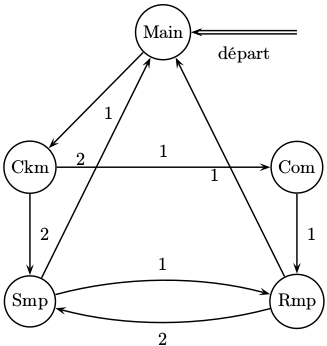
\includegraphics[width=0.5\textwidth]{automate.png}
\end{center}
\iffalse
\begin{center}
	\qquad \begin{psmatrix}
		& & [mnode=circle] Main &\\
		& [mnode=circle] Ckm & & [mnode=circle] Com\\
		& [mnode=circle] Smp & & [mnode=circle] Rmp
	\end{psmatrix}
	\psset{arrows=->,shortput=nab,arrowsize=0.15}
	\ncline{1,3}{2,2}^{$1$}
	\ncline{2,2}{2,4}^{$1$}
	\ncline{2,2}{3,2}^{$2$}
	\ncline{2,4}{3,4}^{$1$}
	\ncarc[arcangle=15]{3,2}{3,4}^{$1$}
	\ncline{3,2}{1,3}^{$2$}
	\ncline{3,4}{1,3}^{$1$}
	\ncarc[arcangle=15]{3,4}{3,2}^{$2$}
	\psset{doubleline=true}
	\ncline{1,4}{1,3}^{départ}
\end{center}
\fi
Nous allons expliquer le comportement principal de chaque type d'agent :
\paragraph{Agent Explorateur :}
Sa mission principale est d'explorer la carte et d'établir une connaissance commune pour tous les agents. Il construit la carte au fur et à mesure dans sa propre table de hachage. Il met à jour sa structure de données personnalisée la disponibilité et la quantité des trésors. Lors de la phase de la communication, tous les agents s'échangent leur carte pour compléter la connaissance. On note que tous les n\oe{}uds de la carte ont un timestamp cela nous permet lors de l'échange de la carte de sélectionner les n\oe{}uds les plus récents s'ils sont présents dans les deux cartes. Une fois la carte est complète, l'agent sélectionne des n\oe{}uds aléatoires dans la carte pour mettre à jour les trésors.

\paragraph{Agent Explorateur des n\oe{}uds plus vieux:}
Cet agent a exactement le même comportement que l'agent explorateur avant la complétion de la carte, cependant lorsque celle-ci est complète son but est d'aller explorer les n\oe{}uds les plus vieux de la carte et non des n\oe{}uds sélectionnés au hasard.

\paragraph{Agent Collecteur :} Avant la complétion de la carte cet agent a exactement le même comportement que les agents explorateurs. Si sa carte est complète, il va chercher les trésors de son type qui sont les plus proches de lui. Si son sac à dos est plein ou bien qu'il ne trouve plus de trésors de son type sur la carte, il vas alors se diriger vers le tanker pour y déposer son butin.

\paragraph{Agent Tanker :} Avant la complétion de la carte cet agent l'agent explore la carte comme les Agents Explorateurs pour accélérer le processus d'exploration. Quand le Tanker a la carte complète, il fixe sa position en calculant la Betweenness centrality de tous les n\oe{}uds du graphe pour que les Collecteurs puissent déposer le trésor. La Betweenness centrality sera expliqué plus en détails dans la section Outils (3.2).

\section{Processus de Communication}

\subsection{Les Processus}
Notre algorithme de communication que nous décrivons ci-dessous a été pour maximiser le nombre de communications entre agents, nous ferons donc tout d'abord une description de l'algorithme, puis une analyse du nombre de messages échangés par un agent lors d'une discussion.\\
\linebreak   
\tab Ici le comportement \texttt{Main} est définit comme le comportement principal de chaque agent, par exemple le \texttt{ExploreBehaviour} pour l'agent explorateur. 
Description de l'algorithme :
\begin{itemize}
\item Après chaque action dans l'environnement (\texttt{Main}), l'agent passe au \texttt{CheckMailBehaviour} pour regarder sa boîte aux lettres. On distingue le cas ou il reçoit des demandes de communication  et ou il ne les reçois pas.

\item Si l'agent n'a rien dans sa boîte après un temps d'attente prédéfinit de 50ms , il envoie une demande de communication à tout les autres Agents avec (\texttt{RequestConnectionBehavior}). il passe ensuite au \texttt{ReceiveMapBehaviour} pour attendre des cartes des autres. Après 50 autres millisecondes, s'il n'en reçoit aucune il revient au \texttt{Main}. Sinon il enverra sa carte à l'agent avec qui il est en communication dans le \texttt{SendMapBehavior} puis fusionnera les cartes pour ensuite revenir au \texttt{Main}.

\item Si l'agent a un message et que celui-ci est moins vieux que 50ms, il passe alors au \texttt{SendMapBehavior} pour envoyer sa carte à l'agent dont il récupère le nom dans le message reçu précédemment. Après cette étape il attend de recevoir la carte de son partenaire dans \texttt{ReceiveMapBehaviour} s'il reçoit la carte dans la limite de temps prédéterminé il pourra ensuite fusionner les deux cartes, et enfin revenir au \texttt{Main}.\\

\end{itemize}

\tab Dans le cadre du projet, seulement les objets sérialisables et les chaînes de caractères sont autorisés dans la communication. C'est la raison pour laquelle nous utilisons une table de hachage et une structure de données manipulant les trésors qui implémente les objets sérialisables. Nous terminons donc par l'analyse du nombre de messages échangé par un agent dans le pire des cas, nous prenons donc le cas ou l'agent ne trouve pas de messages dans sa boite aux lettres : 
\begin{itemize}
  \item Envoie d'un message à tous les autres agents sur la carte (\textbf{n} Agents)
  \item Envoie de la carte à l'agent avec qui il est en communication
\end{itemize}
On note donc que le nombre de messages envoyés dans le pire des cas à chaque communication est \textbf{n+1}. De plus, après chaque mouvement, même si aucun agent ne se trouve dans le rayon de communication de l'agent en question, \textbf{n} messages serons envoyé. Il serait donc possible de grandement réduire le nombre de messages en débutant la communication uniquement lors du blocage de l'agent, mais du fait que les agents peuvent communiquer si et seulement s'ils sont dans le rayon de communication (c'est-à-dire une distance de 2 n\oe{}uds du graphe), cela réduirait grandement le nombre d'échange de cartes, ce qui ne nous semblait pas convenir à notre stratégie d'exploration rapide. 

\begin{center}
	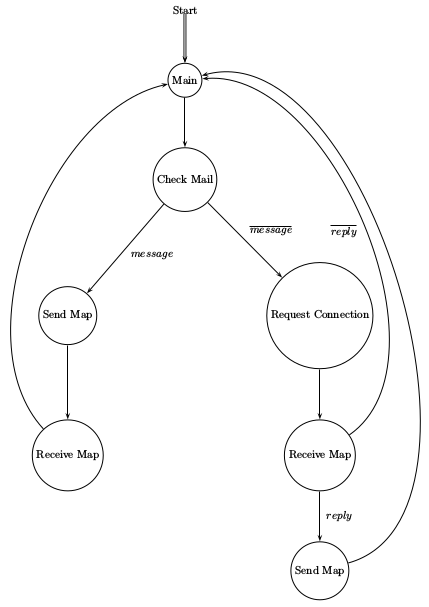
\includegraphics[width=0.8\textwidth]{extend.png}
\end{center}
\iffalse
\begin{center}
	\qquad \begin{psmatrix}
		& & Start&\\
		& & [mnode=circle] Main &\\
		& & [mnode=circle] Check Mail &\\
		& [mnode=circle] Send Map & &  [mnode=circle] Request Connection\\
		& [mnode=circle] Receive Map & &  [mnode=circle] Receive Map\\
		& & &  [mnode=circle] Send Map
	\end{psmatrix}
	\psset{arrows=->,shortput=nab,arrowsize=0.15}
	\ncline{2,3}{3,3}
	\ncline{3,3}{4,2}^{$message$}
	\ncline{3,3}{4,4}^{$\overline{message}$}
	\ncline{4,2}{5,2}
	\ncline{4,4}{5,4}
	\ncline{5,4}{6,4}^{$reply$}
	\ncarc[arcangle=60]{5,2}{2,3}
	\ncarc[arcangle=-75]{5,4}{2,3}^{$\overline{reply}$}
	\ncarc[arcangle=-90]{6,4}{2,3}
	\psset{doubleline=true}
	\ncline{1,3}{2,3}
\end{center}
\fi
\subsection{Les Outils}
\paragraph{Calcul de chemin :} Nous utilisions l'algorithme de Dijkstra en considérant des arêtes ayant toutes le même poids, de ce fait le plus cours chemin sera celui qui a le moins d'arêtes. L'implémentation utilisée de cette algorithme est celle fournie par \texttt{graphStream}. Quant à la recherche du plus court chemin vers plusieurs cases, on applique cet algorithmes vers chacune des cases et on prend le chemin avec la valeur la plus proche.\\
\tab Pour empêcher le blocage des agents explorateurs et collecteurs sur le tanker du fait que celui-ci ne bouge pas. Après que la position du tanker est déterminée nous enlevons ce n\oe{}ud des graphes pour le calcul de Dijkstra ce qui permet aux agents de passer autour du Tanker.\\
\tab \textbf{O(n log(n) + m)} avec n le nombre de n\oe{}uds et m nombre d'arêtes.

\paragraph{Centralisation dans le graphe :} Nous plaçons le Tanker sur le n\oe{}ud de plus haute \href{https://en.wikipedia.org/wiki/Betweenness_centrality}{Betweenness centrality} dans le graphe, c'est-à-dire le n\oe{}ud  qui est dans le plus grande nombre de plus cours chemins entre deux autres n\oe{}uds quelconques du graphe. Pour faire ce calcul nous utilisons l'algorithme fourni par \texttt{graphStream}. Dans la plupart des cas, cette méthode est très efficace. Elle permet de minimiser le chemin que les agents collecteurs ont a faire entre leur trésor et le tanker. L'inconvénient cependant, est que si le graphe se décompose en 2 grands sous-graphes de même taille qui se connectent par un n\oe{}ud unique, une fois le Tanker est placé, il est possible qu'il se trouve sur ce n\oe{}ud unique, les agents ne peuvent donc plus accéder à la partie du graphe dans laquelle ils ne font pas partie du graphe.\\
\tab Une autre méthode a été proposée. C'est de prendre le n\oe{}ud ayant les plus grand nombre de descendants, ce qui permet d'éviter le blocage du cas précédent. Cependant cela nécessiterais de communiquer la position du tanker a tous les agents, ce qui nous semblais être plus coûteux en terme de communication et une moins bonne stratégie.

	
\subsection{Interblocage}
\tab Nous voulions un système robuste pour la gestion de l'interblocage. Il nous semblait en effet très important de minimiser un maximum des risques que deux agents se veuillent se diriger vers une case occupée par un autre agent, c'est pour cette raison que nous avons conçu notre système de communication de façon à ce qu'un échange de carte de fasse le plus souvent possible. Bien que cette méthode soit peu économe en messages, elle minimise les interblocages dans la phase d'exploration car les agents ne se dirigent pas vers les n\oe{}uds qui se trouvent déjà dans leur carte. Nous exploitons cette fonctionnalité de la façon suivante : lorsque deux agents se trouvent à proximité de deux cases, ils échangent leurs carte respectives et de ce fait ne se dirigent pas vers la position où se trouve l'autre agent en communication car celle-ci sera marquée comme explorée.\\
\tab La méthode décrite ci-dessus ne permet cependant pas d'éviter les interblocages dans la phase de récupération des trésors, pour contrer cela lorsque l'un de nos agents n'arrive pas à faire un mouvement, il va sélectionner une case au hasard parmi ses voisins et essayer de s'y déplacer jusqu'à ce que ce soit possible.

\subsection{Amélioration}
Nous pensons qu'il serait possible de grandement améliorer la gestion des interblocages, en effet la sélection d'une case au hasard lorsqu'un agent se bloque est sous optimale lorsque les agents se croisent dans une ligne.\\
\tab Pour accélérer la récupération des trésors il serait possible d'augmenter le nombre de Tanker cela pourrait potentiellement diminuer le temps de trajet des agents des trésors vers le Tanker, on pourrais aussi imaginer un Tanker qui se déplace vers les gants collecteurs.\\
\tab Nous avons aussi pensé à réorienter les agents explorateurs après la complétion de la carte pour bloquer l'agent Wumpus, cela nous permettrait de ne pas nous soucier de la mise à jour de la carte après l'exportation\\
\section{Conclusion}
\tab Vous trouverez ci dessous les performances de notre algorithmes sur l'instance de l'examen de 2017\\
\begin{center}
\begin{tabular}{lll}
   Instance2017 & Trésors & Diamants \\
   Total & 280 & 140\\
   Ramassé & 202 & 128 \\
\end{tabular}
\end{center}
\tab
En conclusion notre méthode remplie le critère de récupération des trésors sur la carte fonctionne ramassage rapide 
exploration très rapide vulnérabilités 
blocage sous optimale .



	
\end{document}
% !TeX program = xelatex